%
% Modified by Sameer Vijay
% Last Change: Wed Jul 27 2005 13:00 CEST
%
%%%%%%%%%%%%%%%%%%%%%%%%%%%%%%%%%%%%%%%%%%%%%%%%%%%%%%%%%%%%%%%%%%%%%%%%
%
% Sample Notre Dame Thesis/Dissertation
% Using Donald Peterson's ndthesis classfile
%
% Written by Jeff Squyres and Don Peterson
%
% Provided by the Information Technology Committee of
%   the Graduate Student Union
%   http://www.gsu.nd.edu/
%
% Nothing in this document is serious except the format.  :-)
%
% If you have any suggestions, comments, questions, please send e-mail
% to: ndthesis@gsu.nd.edu
%
%%%%%%%%%%%%%%%%%%%%%%%%%%%%%%%%%%%%%%%%%%%%%%%%%%%%%%%%%%%%%%%%%%%%%%%%

%%%%%%%%%%%%%%%%%%%%%%%%%%%%%%%%%%%%%%%%%%%%%%%%%%%%%%%%%%%%%%%%%%%%%%%%
%
% Appendix
%
%%%%%%%%%%%%%%%%%%%%%%%%%%%%%%%%%%%%%%%%%%%%%%%%%%%%%%%%%%%%%%%%%%%%%%%%

\chapter{Publications}
\label{appendix: pubs}

Included in this appendix are the publications that have come from this work.



\section{Lifetime measurements of excited states in $^{15}$O}

\cite{Frentz2021} B.\ Frentz, A.\ Aprahamian, A.\ M.\ Clark, R.\ J.\ Deboer, C.\ Dulal, J.\ D.\ Enright, J.\ G{\"{o}}rres, S.\ L.\ Henderson, J.\ D.\ Hinnefeld, K.\ B.\ Howard, R.\ Kelmar, K.\ Lee, L.\ Morales, S.\ Moylan, Z.\ Rahman, W.\ Tan, L.\ E.\ Weghorn, and M.\ Wiescher. Lifetime measurements of excited states in $^{15}$O. \textit{Phys.\ Rev.\ C,} 103(4):1-10, 2021. ISSN 24699993. doi: 10.1103/PhysRevC.103.045802.

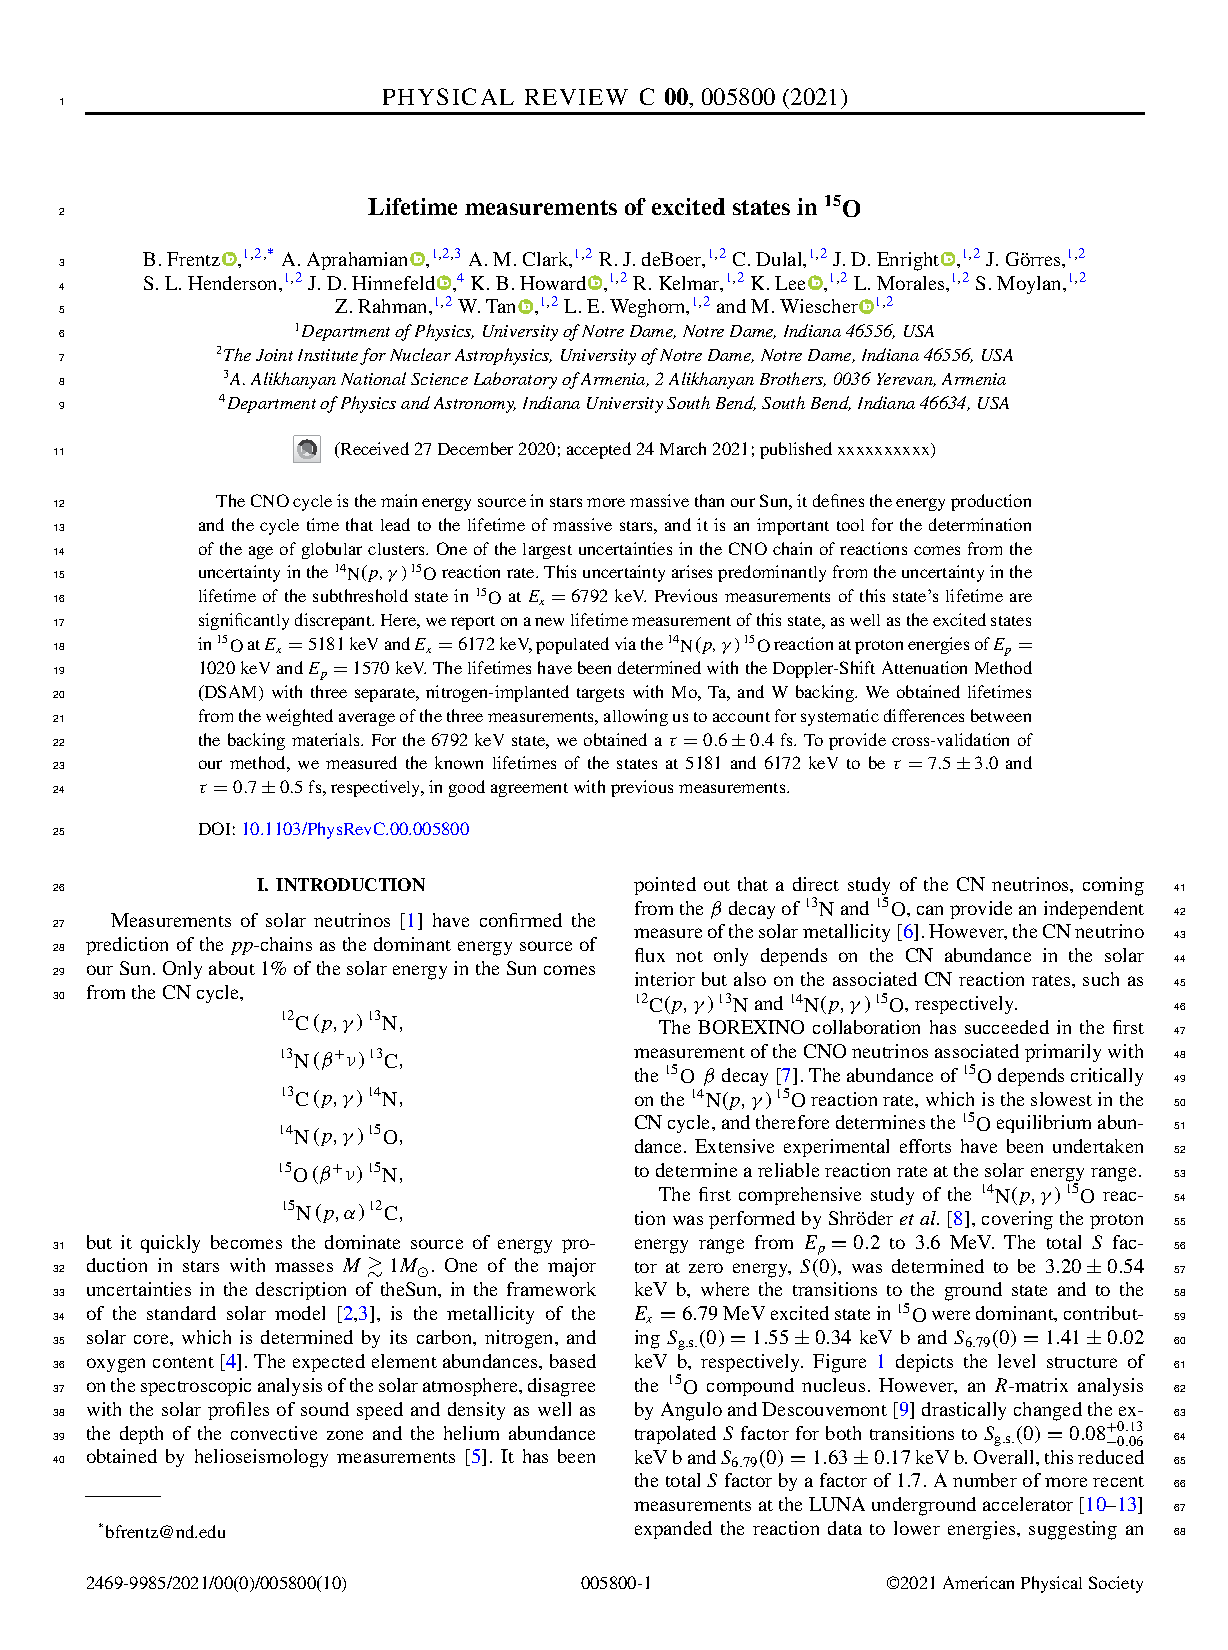
\includepdf[pages=-,pagecommand={},width=\textwidth]{./publications/lifetimesPaper.pdf}


\section{Astrophysical $S$-Factor measurement of the $^{14}$N$(p,\gamma)^{15}$O reaction in the CNO cycle}

\textbf{This paper is currently in preparation.}

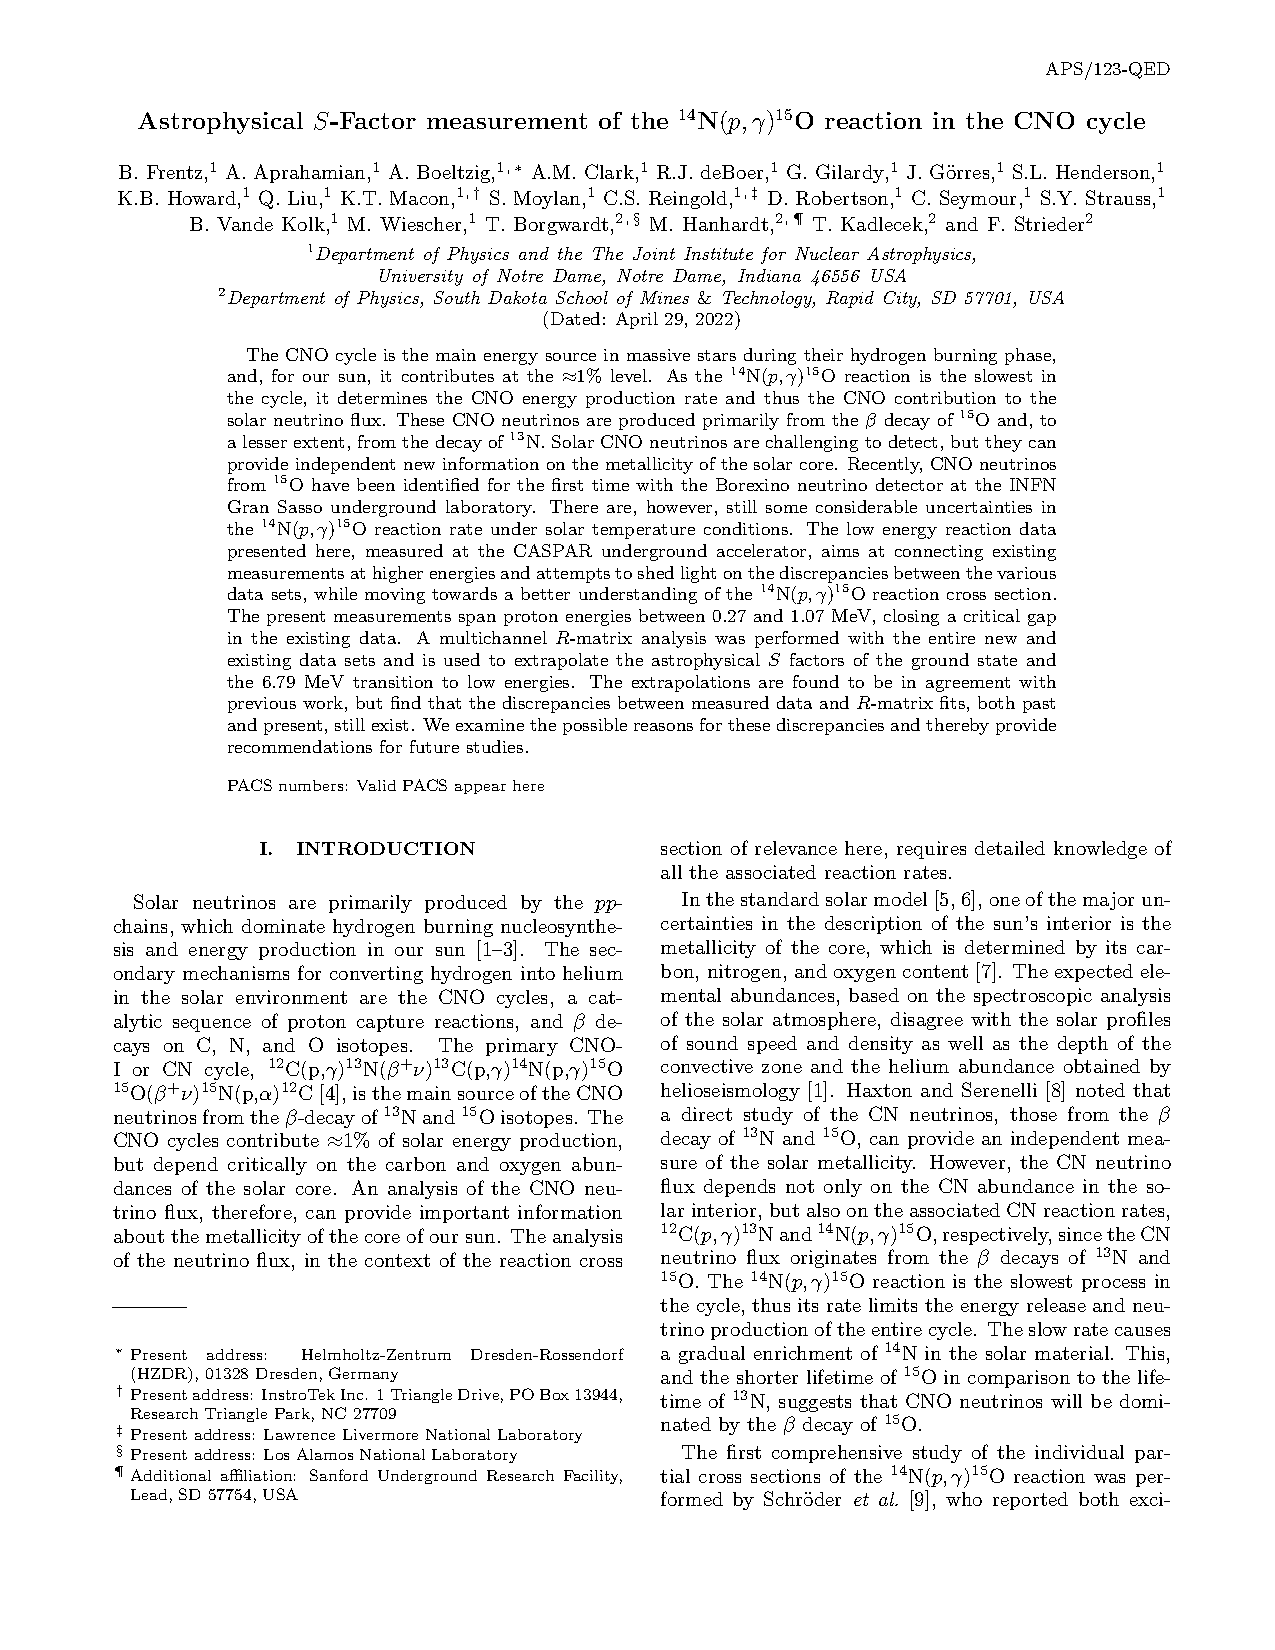
\includepdf[pages=-,pagecommand={},width=\textwidth]{./publications/crossSectionPaper.pdf}

% % uncomment the following lines,
% if using chapter-wise bibliography
%
% \bibliographystyle{ndnatbib}
% \bibliography{example}
